\clearpage
\appendices
\section{Additional Experimental Results}

\subsection{Simulation Experiments}

\noindent\textbf{Numerical results.} We report the numeric values for the success rates on LIBERO benchmark in Table~\ref{tab:libero-results}. All methods use 20$\%$ of the demonstration trajectories except the oracle. See Sec.~\ref{sec:app:unipi} for details about the comparisons on UniPi and UniPi-Replan.

\noindent\textbf{Attention map visualization of track-guided policy.}
To demonstrate how tracks guide the policy, we visualize the attention maps between the spatial CLS token and RGB tokens in the spatial transformer of BC and our method. Figure~\ref{fig:policy-attention-map} demonstrates that our method effectively focuses on the relevant spatial regions, as specified by the textual instructions. Specifically, it attends to the cream cheese, bowl, and wine bottle in the respective example tasks, while BC is usually distracted by the irrelevant regions, highlighting the superior capability of the tracks as better task prompts.


\subsection{Discussions on the UniPi Baselines}\label{sec:app:unipi}

UniPi~\cite{du2023unipi} proposes to train a language-conditioned video diffusion model $f_\theta$ during video pre-training. During policy learning, given the initial image observation $o_0$ and the language $l$, UniPi first generates all future frames $\Tilde{o}_1, \dots \Tilde{o}_{T-1} = f_\theta (o_0, l)$ and then learns an inverse dynamics model that predicts the action at each time step $a_t = \pi(o_t, \Tilde{o}_{t+1})$. UniPi then executes the actions open-loop. However, training a diffusion model to predict the full video can be computation intensive, As such, the UniPi implementation in our paper follows the one in \citet{Ko2023Learning}, where we predict $N=7$ future frames as the sub-goals for the policy, denoted as $\Tilde{o}_1, \dots \Tilde{o}_N$. During training, we evenly sample $N$ frames in an episode for training the video prediction model. During policy learning, we train a goal-conditioned policy $\pi(a_t, \text{done} | o_t, \Tilde{o}_{i})$, where $i\in {1, \dots N}$ is the image sub-goal and $t$ denotes the current timestep. The policy additionally predicts a done flag to determine when it should switch from the current sub-goal $\Tilde{o}_i$ to the next sub-goal $\Tilde{o}_{i+1}$. ATM's superiority over UniPi can be attributed to two reasons. First, ATM uses a more structured sub-goal representation of point trajectories. Second, ATM performs closed-loop inference, proposing a new sub-goal at each time step, while UniPi's video diffusion process is too slow to be referenced at every time step. 

\begin{table}[ht]
    \centering
    \caption{Computation cost and inference time for different methods on a V100 GPU. ATM performs trajectory generation instead of predicting high-dimensional frames, making it the most computationally efficient and feasible for closed-loop control. UniPi employs a video diffusion model for open-loop future goal generation at the beginning, demanding significantly higher computational resources. UniPi-Replan generates fewer frames than UniPi using a smaller model, resulting in marginally faster generation. However, its use in closed-loop control remains computationally prohibitive.}
    \begin{tabular}{c c c c}
    \toprule
    \multirow{2}{*}{Computation} & \multicolumn{2}{c}{Close-Loop} & Open-Loop \\
    % \cline{2-4}
     &  ATM & UniPi-Replan & UniPi\\
    \midrule
    TFLOPS per generation        & 1.56 & 13.09 & 39.29 \\
    Time per generation (s)  & 0.015 & 4.51   & 8.14  \\
    \bottomrule
    \end{tabular}
    \label{tab:runtime}
\end{table}

To train the UniPi policy, we sample $o_{i}$ from a future frame $o_{t}$ where $t \in [t, t+t_{max}]$. We choose $t_{max}$ for each task suite ($t_{max} = 16$ for LIBERO-Object and LIBERO-Spatial, $t_{max} = 50$ for LIBERO-Goal and LIBERO-Long). To mitigate dataset imbalance when learning the done flag, we sample $o_{i}$ as the next frame 10\% of the time. We perform MSE regression on both the action $a_t$ and done.

In order to decouple the two advantages of ATM over UniPi additionally compare with a UniPi variation where we train the video prediction model to predict a fixed time step into the future $\Tilde{o}_{t+H}= f_\theta(o_t)$ for every $H$ steps of policy execution, where $H=8$. As this variation replans the sub-goal more frequently, we call this method \textit{UniPi-Replan}, similar to the implementation in~\cite{black2023zero}. The results are shown in Table~\ref{tab:libero-results}. Surprisingly, we found that this variation performs even worse than UniPi. \textbf{We thus draw the conclusion that a structured sub-goal representation can be much more effective than an image sub-goal.}  The reason is that predicting an image goal at a fixed future time step can be a difficult objective for the video prediction model, leading to inconsistent subgoals. Please refer to the failure videos of various baselines on our website. Additionally, this method requires heavy computation. A comparison of the computation needed is shown in Table~\ref{tab:runtime}. Due to the computation cost, we only evaluate UniPi-Replan on LIBERO-Object and LIBERO-Goal and report the average success across 10 trials on one policy training random seed.




\begin{figure*}[ht]
    \centering
    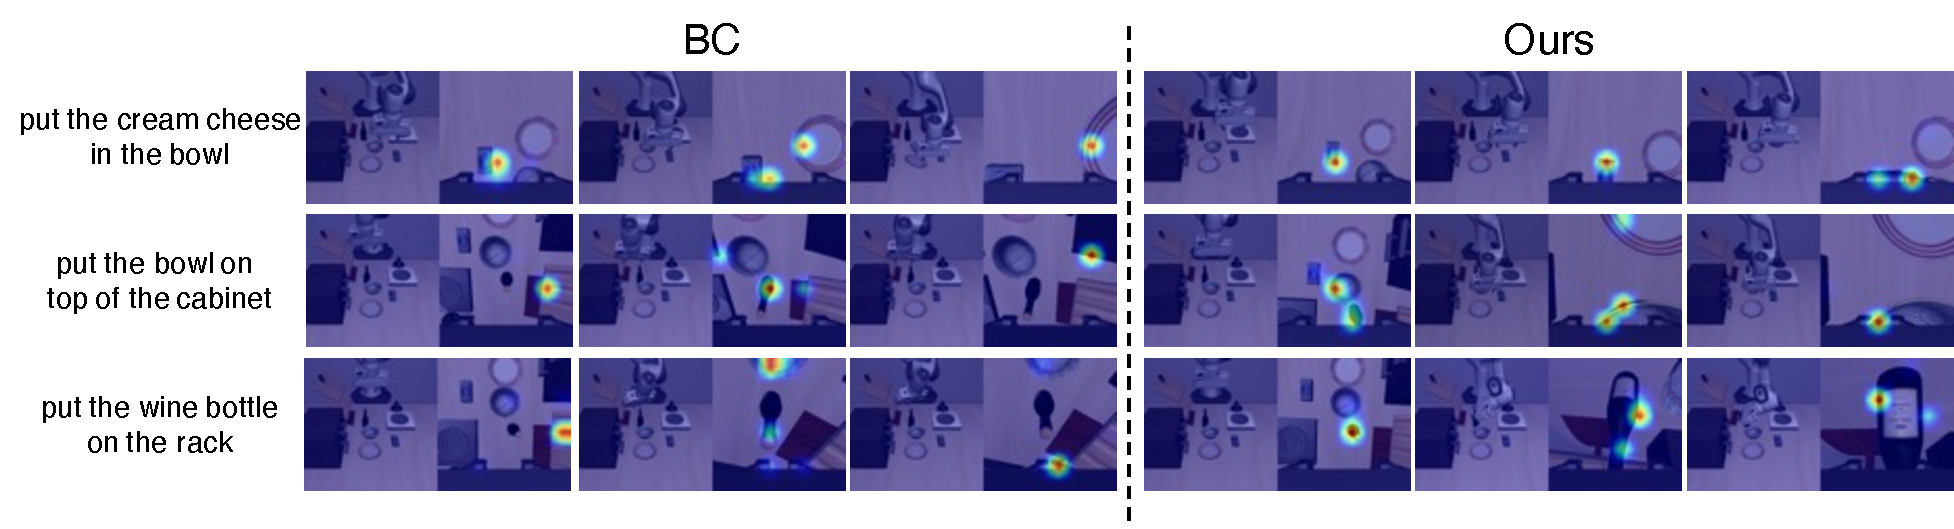
\includegraphics[width=0.95\linewidth]{fig/attention_map.pdf}
    \caption{The attention maps of BC and Ours in the spatial transformer. We extract the attention weights between spatial CLS tokens and RGB tokens, highlighting the policy's focus on specific spatial regions during decision-making. The heatmaps reveal our policy's targeted attention on task-relevant areas, in contrast to BC's tendency to focus on irrelevant backgrounds. This underscores the effectiveness of input tracks in the spatial transformer as good task prompts, guiding the CLS token to attend to appropriate areas.}
    \label{fig:policy-attention-map}
\end{figure*}

\begin{table*}[ht]
  \centering
  \caption{Average success rate on LIBERO benchmark. Our method performs consistently better than all the baselines across all suites. UniPi-Replan is only evaluated for a single seed due to the computation cost.}
  \begin{tabular}{@{}ccccccc@{}}
    \toprule
    Method & Libero-Spatial & Libero-Object & Libero-Goal & Libero-Long & Libero-90 \\
    \midrule
    BC-Full-Trainset (Oracle) & $71.83\pm3.70$ & $71.00\pm7.97$ & $76.33\pm1.31$ & $24.17\pm2.59$ & - \\
    \midrule
    BC & $39.00\pm8.20$ & $51.83\pm13.54$ & $42.50\pm4.95$ & $16.67\pm3.66$ & $29.78\pm1.14$ \\
    R3M-finetune~\cite{nair2023r3m} & $49.17\pm3.79$ & $52.83\pm2.25$ & $5.33\pm1.43$ & $9.17\pm2.66$ & $9.59\pm0.27$ \\
    VPT~\cite{baker2022vpt} & $37.83\pm4.29$ & $19.50\pm0.82$ & $3.33\pm2.36$ & $3.83\pm1.65$ & - \\
    UniPi~\cite{du2023unipi,Ko2023Learning} & $\bf 69.17 \pm 3.75$ & $59.83 \pm 3.01$ & $11.83 \pm 2.02$ & $5.83 \pm 2.08$ & - \\
    UniPi-Replan~\cite{black2023zero} & - & 31.00 & 3.00 & - & - \\
    ATM (Ours) & $68.50\pm1.78$ & $\bf 68.00\pm6.18$ & $\bf 77.83\pm0.82$ & $\bf 39.33\pm15.80$ & $\bf 48.41\pm2.09$ \\
    \bottomrule
  \end{tabular}
  \label{tab:libero-results}
\end{table*}
 

\begin{figure}[ht]
  \centering
  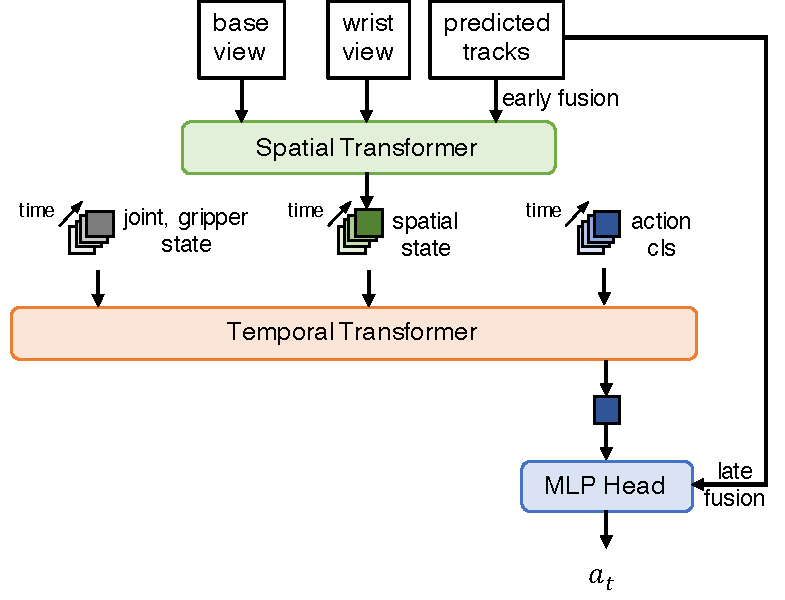
\includegraphics[width=0.9\linewidth]{fig/track_policy_app_simpler.pdf}
  \caption{To summarize spatial information, we perform self-attention on a sequence consisting of all views' track and image patches and a CLS token. To integrate information across time, we perform casual self-attention between spatial CLS token, proprioception, and an action CLS token per timestep. To regress actions, we concatenate each timestep's action CLS token and proposed tracks. }
  \label{fig:arch-appendix}
\end{figure}

\begin{figure}[ht]
  \centering
  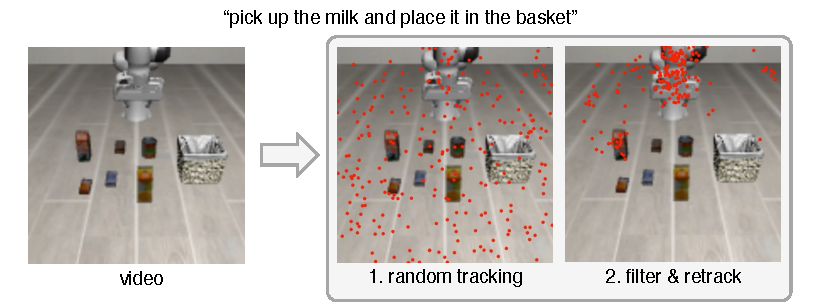
\includegraphics[width=\linewidth]{fig/filtering.pdf}
  \caption{Given a video (left), we query 1000 randomly sampled points using an off-the-shelf TAP model (middle), where each colored dot represents the starting position of a track. We then filter the tracks using a heuristic of their position displacement across the video and re-sample around these points (right). We can see that extracted tracks are concentrated around informative objects, such as the robot's gripper and manipulation targets.}
  \label{fig:filtering}
\end{figure}


\subsection{Applying ATM to Diffusion Policy}
In addition to the transformer policy adopted from the original LIBERO paper~\cite{liu2023libero}, our ATM can also be integrated with the state-of-the-art Diffusion Policy~\cite{Chi2023diffusion}. Specifically, we implement an ATM Diffusion Policy by using predicted tracks as input conditions. Both the standard and ATM-based Diffusion policies are trained with 20\% of the data from LIBERO, in the same setting as the experiment in Figure~\ref{fig:sim_exp}.

As shown in Table~\ref{tab:diff-policy}, the standard Diffusion Policy achieves impressive results on the LIBERO benchmark, even with limited training data, confirming its status as the state-of-the-art imitation policy. Moreover, the ATM Diffusion Policy consistently outperforms the standard model, highlighting our framework's versatility and effectiveness across different policy architectures.


\begin{table*}[ht]
  \centering
  \caption{Detailed results of Diffusion policy on LIBERO. The Diffusion policy can be further improved by our method, suggesting that our Any-point Trajectory Modeling framework is an important building block to apply to any policy model.}
  \begin{tabular}{@{}cccccc@{}}
    \toprule
    Method & Libero-Spatial & Libero-Object & Libero-Goal & Libero-Long & Libero-90 \\
    \midrule
    Diffusion Policy & $67.67\pm1.25$ & $78.00\pm2.45$ & $35.00\pm3.74$ & $37.33\pm2.05$  & $33.85\pm1.71$ \\
    ATM Diffusion Policy & $79.00\pm3.74$ & $81.00\pm2.45$ & $58.67\pm4.64$ & $44.00\pm6.38$ & $62.89\pm1.10$ \\
    \bottomrule
  \end{tabular}
  \label{tab:diff-policy}
\end{table*}


\subsection{Human-to-robot Transfer Details}
To demonstrate the potential of ATM to leverage out-of-domain videos, we design human-to-robot transfer tasks in three different settings: 1) deformable object: \textit{fold the cloth and pull it to the right}, 2) long horizon: \textit{put the tomato into the pan and close the cabinet door}, and 3) tool using: \textit{use the broom to sweep the toys into the dustpan and put it in front of the dustpan}.
We collect 10 robot teleportation trajectories (action-labeled) and 100 human manipulation videos (action-free). We compare three methods: 1) behavioral cloning only with 10 action-labeled robot demos, 2) ATM, training track transformer with only 10 robot demos, and 3) ATM, training a track transformer with both action-free human and action-labeled robot data.
For each task, we train each method with three different random seeds, evaluate them in the real world 10 times, and report the average success rate in Table~\ref{tab:human-robot-result}.

\noindent\textbf{Human-to-Robot visualization.}
The detailed video visualizations of human-to-robot skill transfer are shown in Figure~\ref{fig:human_video_supp}. Due to limited training samples, the track transformer trained with only 10 robot videos fails to predict the future point trajectories, leading to low success rates. In contrast, the trajectory model trained with human videos generates high-quality tracks in each frame, guiding the agent to successfully complete the task with only 10 action-labeled trajectories. This indicates our any-point trajectory modeling enables to transfer the motion prior from cross-embodiment videos to robot skills, which significantly improves policy learning.

Furthermore, we visualize the attention maps of Track Transformers trained with or without human videos in Figure~\ref{fig:tt-attention-map}. Track Transformer trained with human videos (bottom row) displays well-defined attention heatmaps that primarily focus on the object and robot arm. Conversely, the attention maps from the model trained without human videos (middle row) are notably more dispersed, often incorrectly focusing on background areas. This comparison highlights the effectiveness of our ATM in leveraging prior knowledge from human videos, facilitating successful cross-embodiment imitation learning.


\begin{table*}[ht]
\begin{minipage}[c]{0.48\textwidth}
\makeatletter\def\@captype{table}
\centering
\caption{Hyperparameters of track transformer training.}
\begin{tabular}{@{}cc@{}}
    \toprule
    Hyperparameters & Track Transformer \\
    \midrule
    epoch & 100  \\
    batch size &  1024  \\
    optimizer & AdamW  \\
    learning rate & 1e-4  \\
    weight decay & 1e-4 \\
    lr scheduler & Cosine  \\\
    lr warm up & 5 \\
    clip grad & 10 \\
    point sampling & variance filtering \\
    number of points & 32 \\
    track length & 16 \\
    track patch size & 4 \\
    image mask ratio & 0.5 \\
    augmentation & ColorJitter,RandomShift \\
    \bottomrule
\end{tabular}
\label{tab:tt-hyperparameter}
\end{minipage}
\begin{minipage}[c]{0.48\textwidth}
\makeatletter\def\@captype{table}
\centering
  \caption{Hyperparameters of policy training.}
  \begin{tabular}{@{}cc@{}}
    \toprule
    Hyperparameters & Policy  \\
    \midrule
    epoch & 100  \\
    batch size &  512  \\
    optimizer &  AdamW  \\
    learning rate & 5e-4  \\
    weight decay & 1e-4 \\
    lr scheduler & Cosine  \\
    lr warm up & 0 \\
    clip grad & 100 \\
    point sampling & grid \\
    number of points & 32 \\
    track length & 16 \\
    frame stack & 10 \\
    augmentation & ColorJitter,RandomShift \\
    \bottomrule
  \end{tabular}
  \label{tab:policy-hyperparameter}
\end{minipage}
\end{table*}


\begin{figure*}
    \centering
    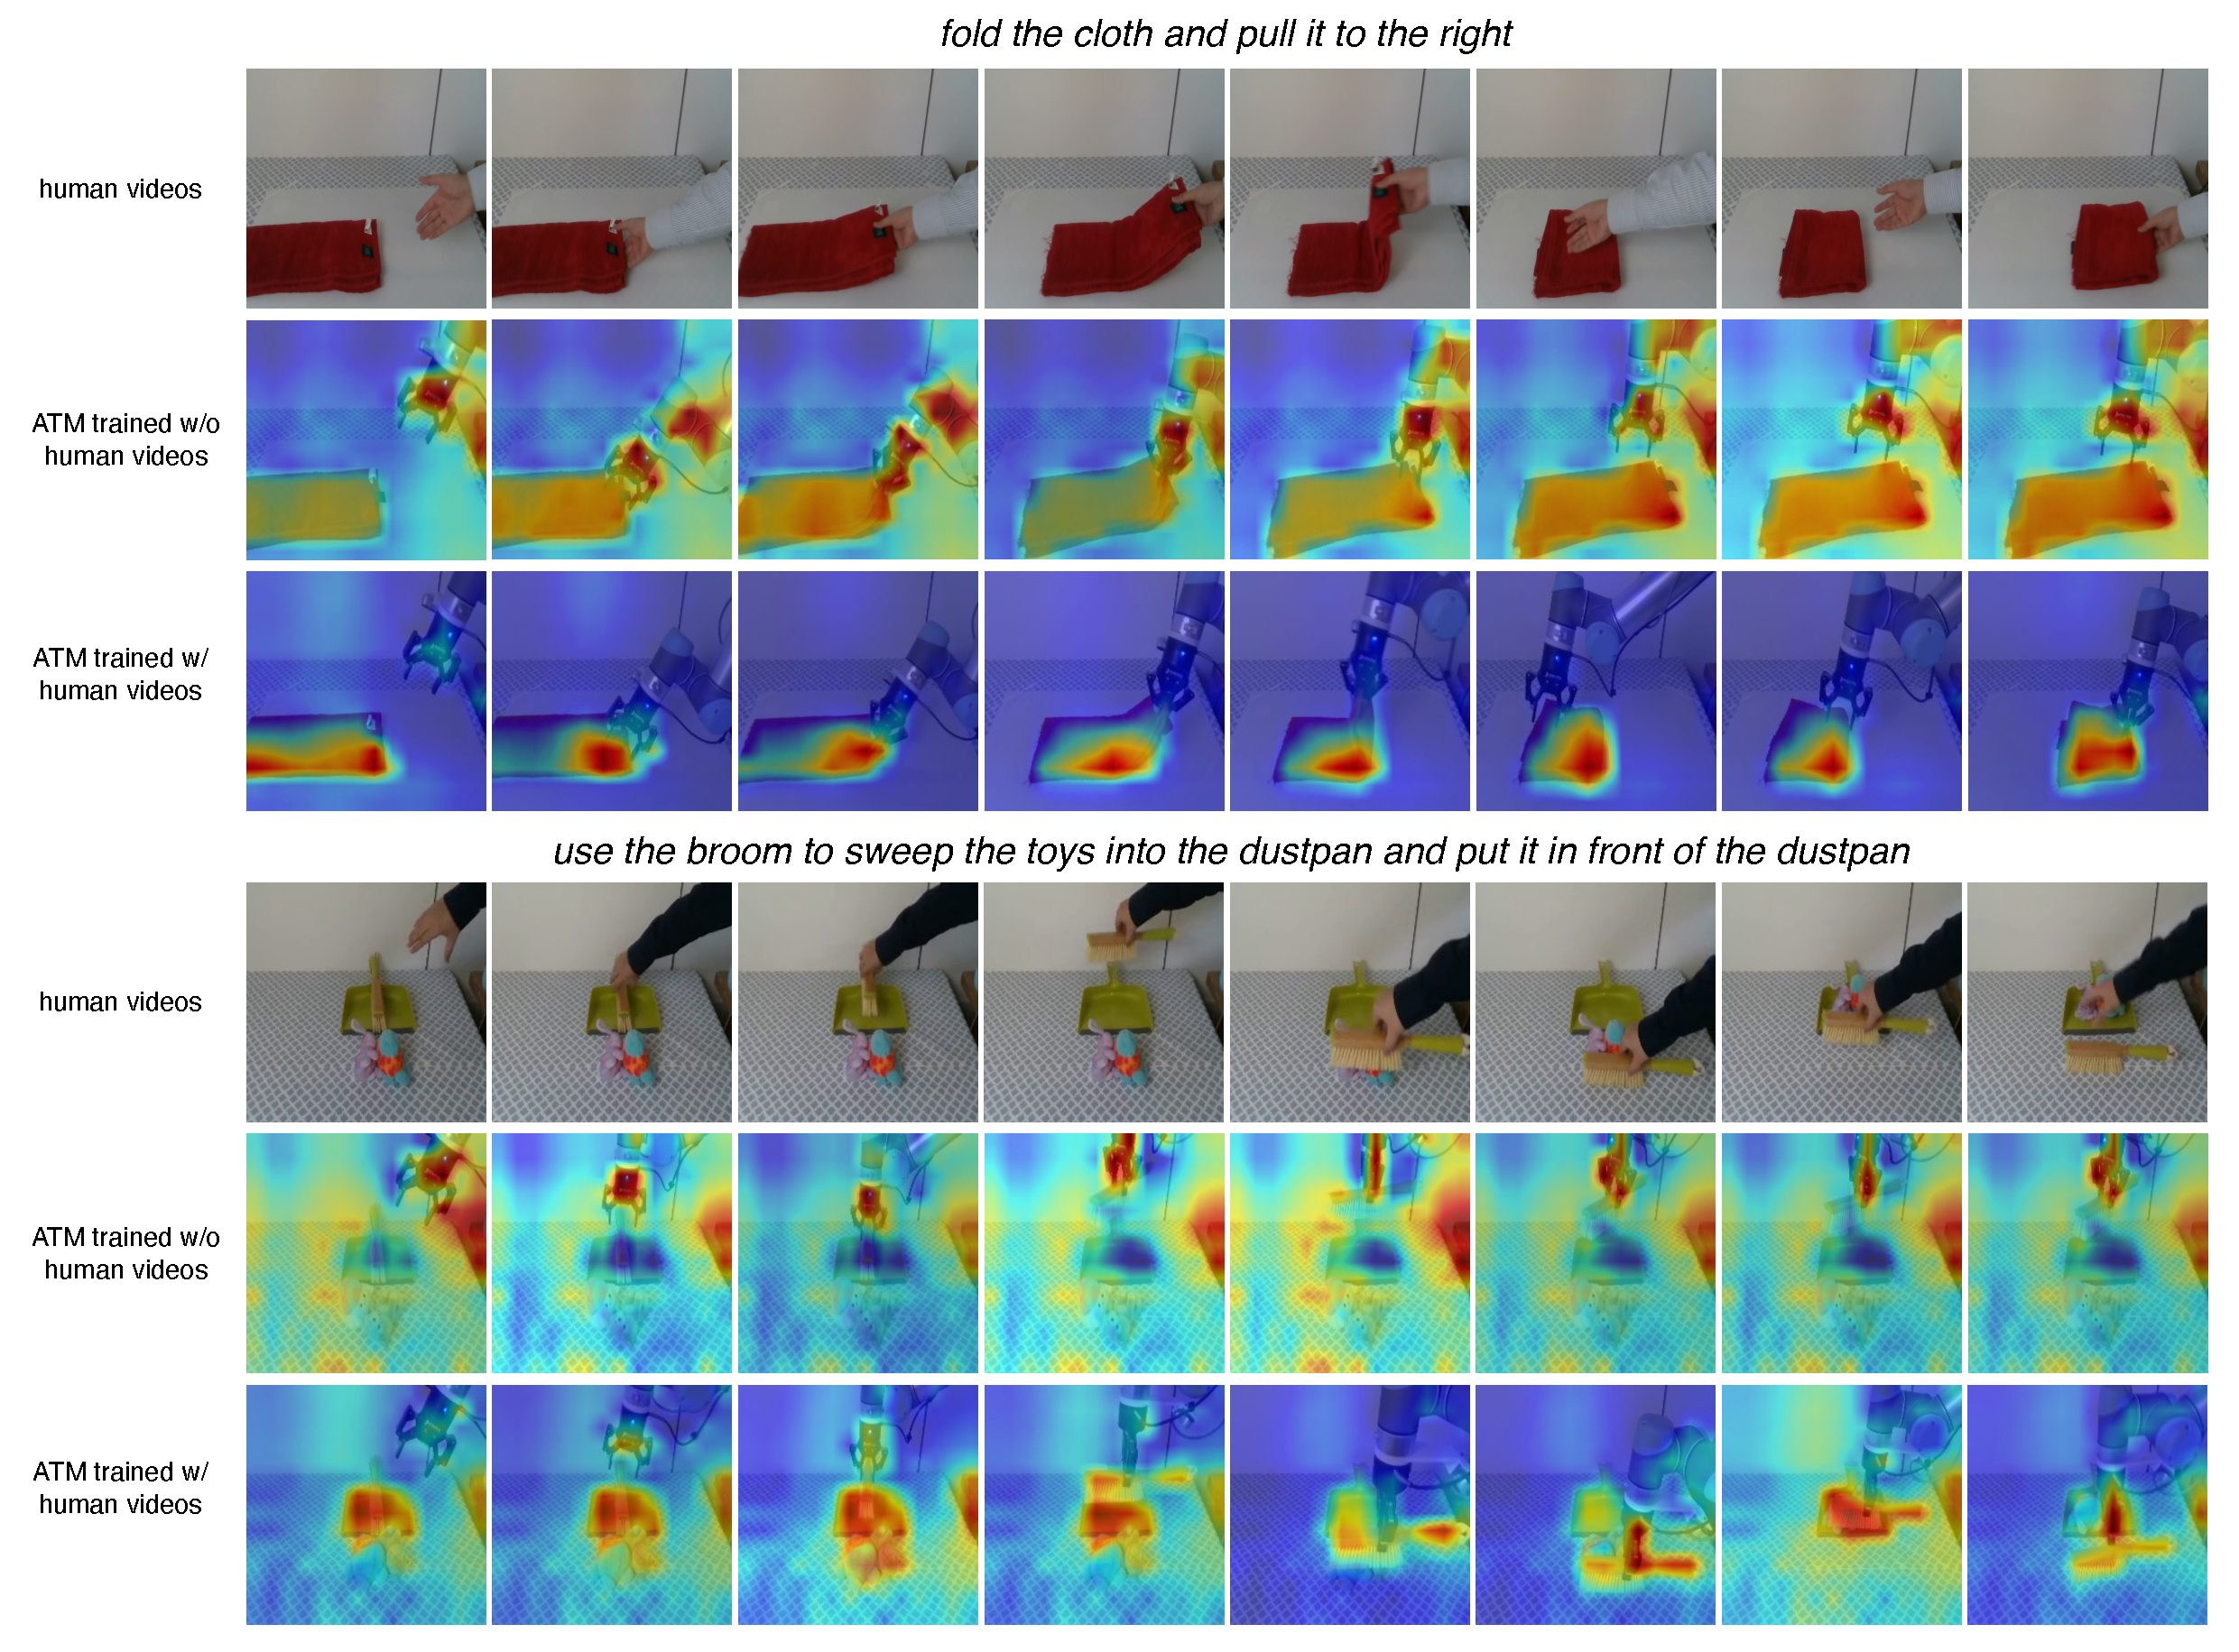
\includegraphics[width=0.95\linewidth]{fig/human_video_attn_rebuttal.pdf}
    \caption{Attention maps of Track Transformer trained with and without human videos. Including large-scale human video leads to much clearer attention maps, focusing on the object and robot arm, while training without human videos will attend to incorrect areas such as background walls.}
    \label{fig:tt-attention-map}
\end{figure*}

\begin{figure*}[ht]
    \centering
    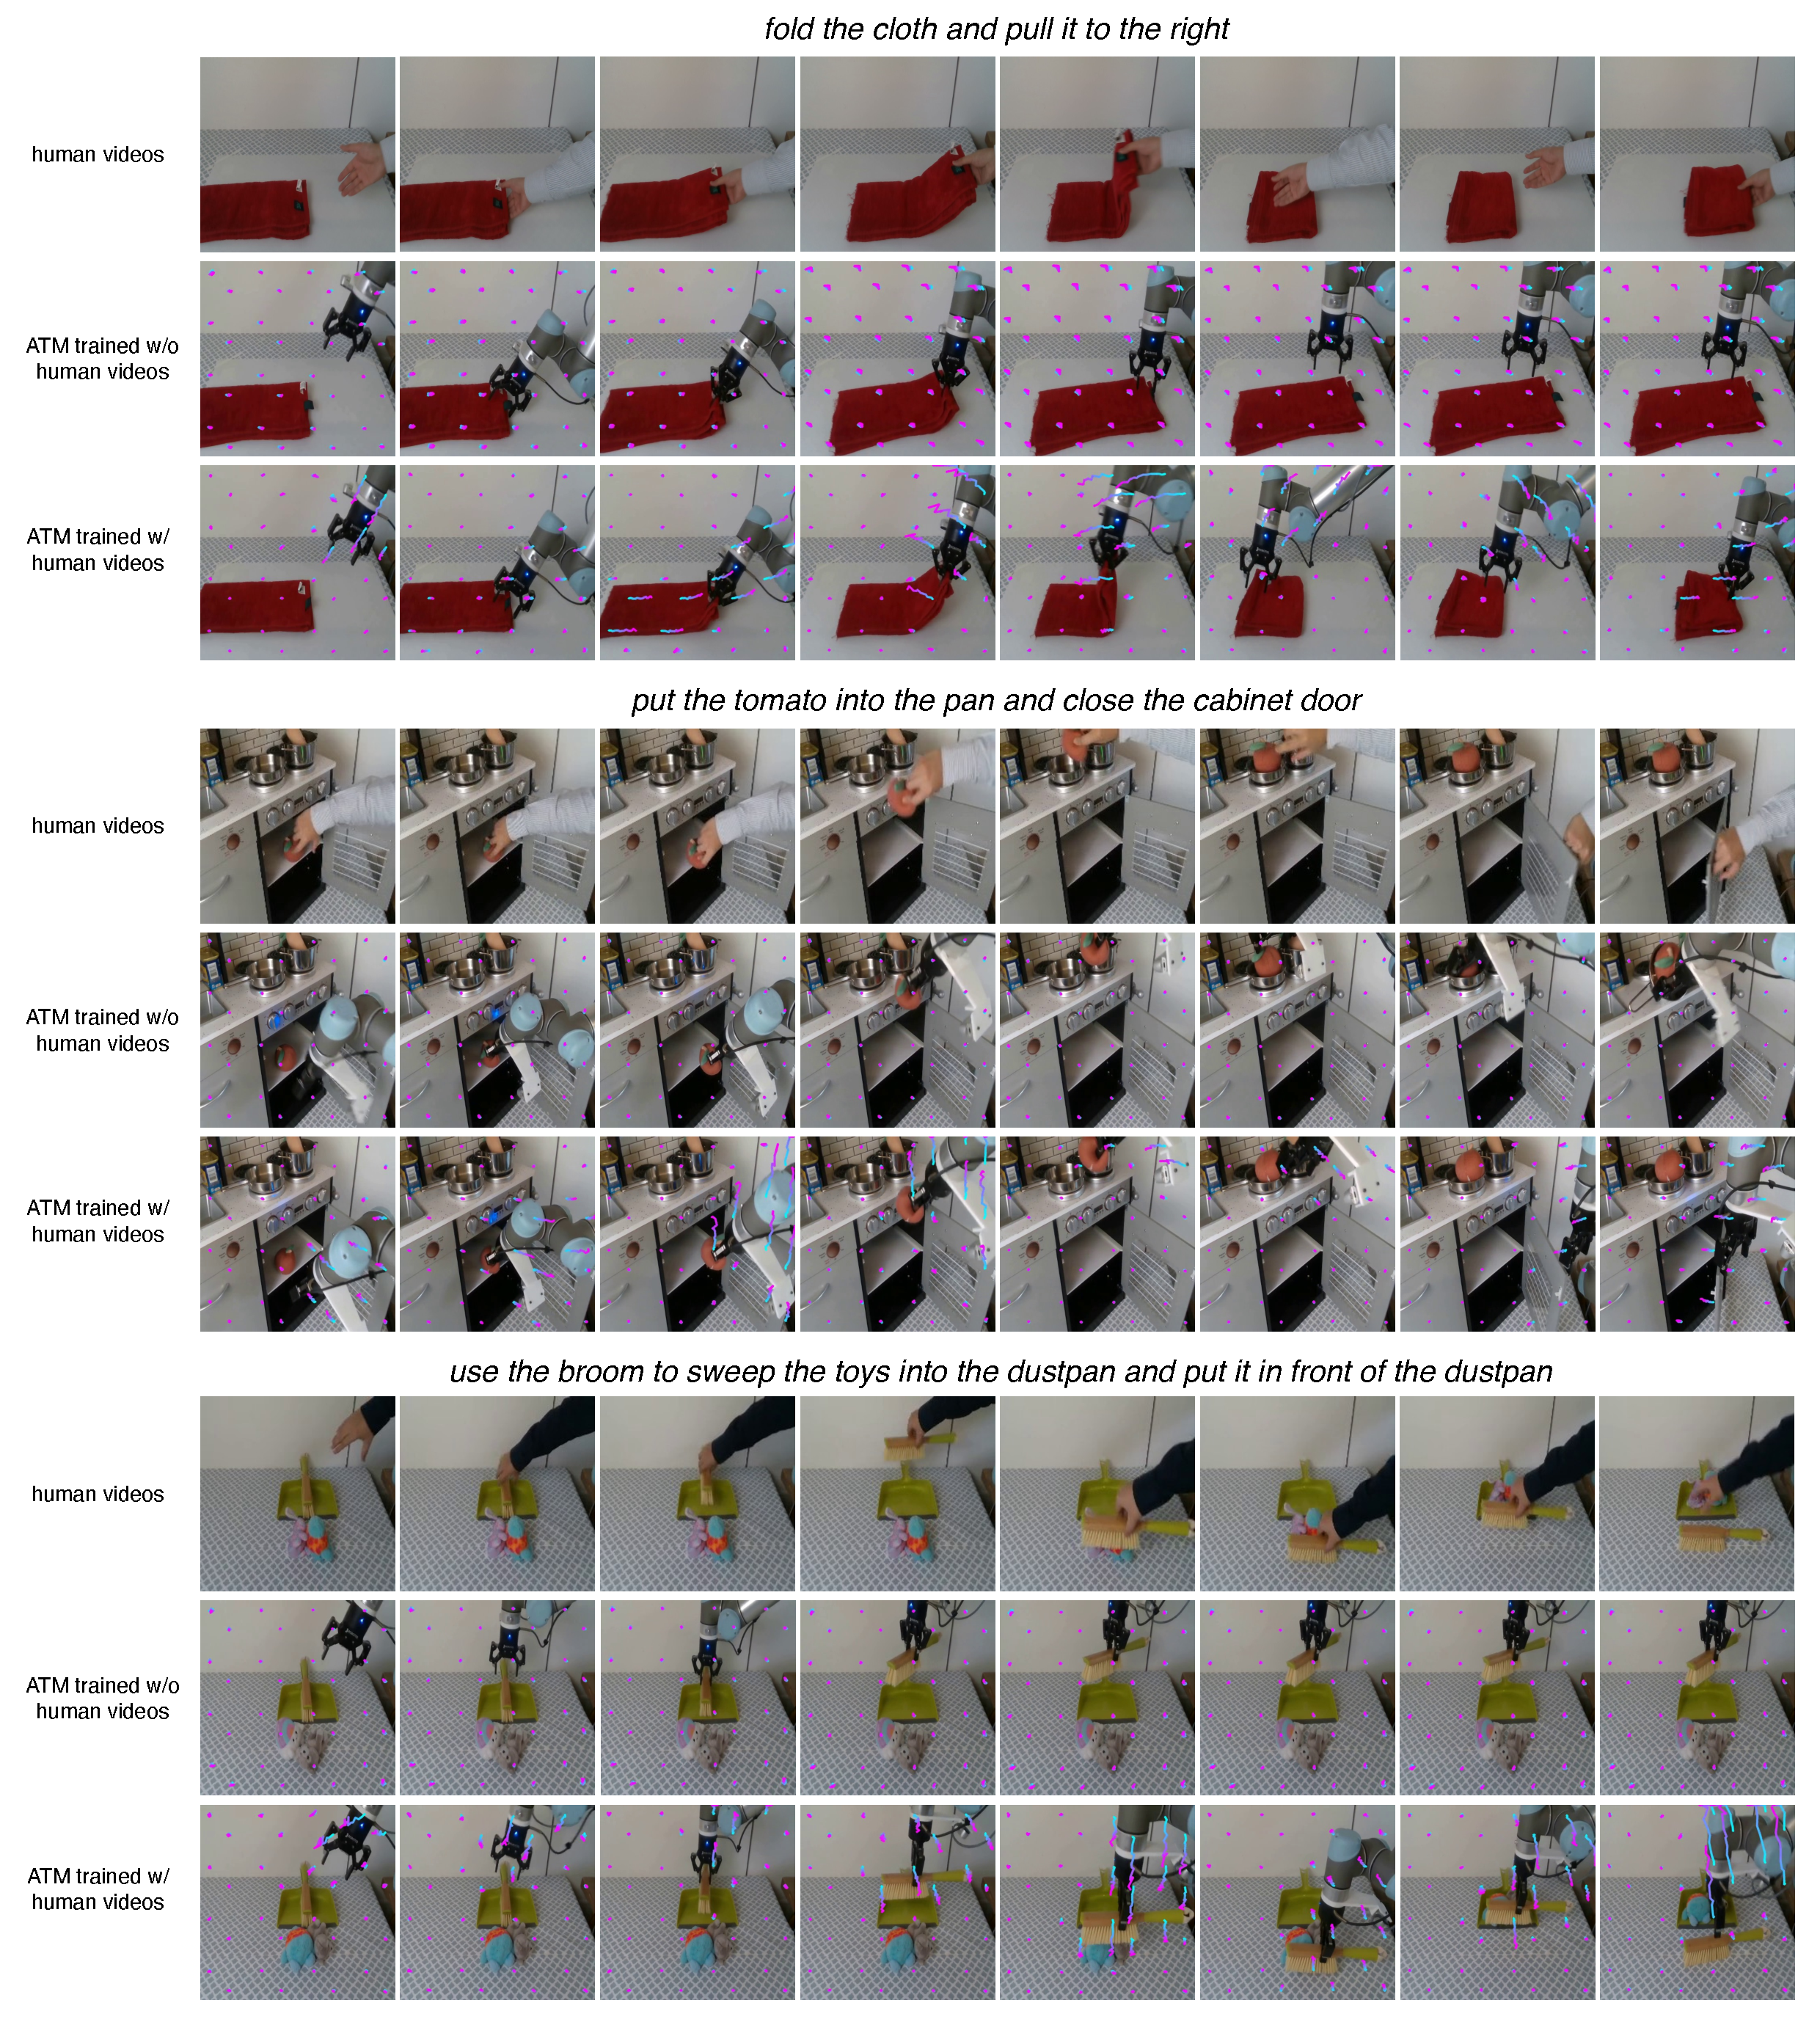
\includegraphics[width=\linewidth]{fig/human_video_supp_3task.pdf}
    \caption{The visualizations of human demos and rollout videos of ATM policies trained with and without human data. We can see that ATM is able to take advantage of out-of-domain videos, i.e., human videos, to generate more precise tracks, resulting in better policy performance.}
    \label{fig:human_video_supp}
\end{figure*}


\section{Implementation Details}
\subsection{Policy Architecture}~\label{sec:app:policy-arch}
We include a more detailed visual of the ViT-T~\cite{liu2023libero, kim2021vilt} policy used in our experiments in Figure~\ref{fig:arch-appendix}. The input to our policy is a set of temporally stacked images across multiple views $o_t \in \mathbb{R}^{V\times T \times C\times H\times W}$, and proprioception $p_t \in \mathbb{R}^{D_p}$. To process these inputs, ViT-T consists of three stages: \\

\noindent\textbf{Spatial Encoding}: We encode all modalities at each timestep. We first leverage the frozen track transformer to propose a set of tracks for all $V$ frames in $o_t$. We then project each modality with modality-specific encoders into a shared embedding space $\mathbb{R}^D$. Each modality's tokens are embedded using a shared learned modality token, and modality-specific positional embeddings. We then concatenate tokens across all modalities and views with a learned spatial CLS token, and perform self-attention on the sequence. We extract the spatial CLS token as the representation. \\

\noindent\textbf{Temporal Decoding}: We process the encoded modalities across timesteps into actions. We first project the proprioception at each timestep into the same shared embedding space $\mathbb{R}^D$. We then interleave the encoded proprioception, the spatial CLS token, and a learned action CLS token across timesteps into a sequence, before performing causally-masked self attention between the sequence. \\

\noindent\textbf{Action Head}: We treat each timestep's output independently and parameterize actions using an MLP. For each timestep, we take the action CLS token, and fuse the CLS token with the reconstructed tracks of the current timestep. \\

\subsection{Efficient Training with Point Filtering}\label{sec:app:track-filter}
We adopt a heuristic to filter out the static points in the background and then utilize an off-the-shelf tracking model to generate the corresponding tracks of the large-motion points. The visualization of the sampled points before and after the filtering process is shown in Figure~\ref{fig:filtering}.


\subsection{Training Details}~\label{sec:app:train-detail}
We list the training hyperparameters for the track transformer and track-guided policy in Table~\ref{tab:tt-hyperparameter} and \ref{tab:policy-hyperparameter}, which are fixed for all experiments on LIBERO benchmark. We train all models on 4 A100 GPUs with DeepSpeed strategy.

We train the track transformer using the ground truth tracks generated by CoTracker~\cite{karaev2023cotracker} and save the checkpoint with the lowest validation loss as our final model to apply for policy learning. We do not incorporate frame stacking for track transformer to avoid causal confusion~\cite{wen2022primenet}. 

We train policies using the expert demonstrations provided by LIBERO, which is collected by human experts through teleoperation with 3Dconnexion Spacemouse~\cite{liu2023libero}. Since the validation loss in behavioral cloning is not always reliable, we save the checkpoint of the last epoch for online rollout evaluation.
